\chapter{基于属性保持对抗网络的零样本物体分类方法}

零样本物体分类问题是指当训练集和测试集包含的图像类别不同时,模型仍然能够准确地对训练过程中从未见过类别的图像进行分类。目前,虽然主流的零样本物体分类方法都是基于嵌入映射的模型,但是这类方法不可避免地存在一定的语义丢失(semantic loss)。语义丢失是指在零样本分类的训练过程中,模型往往选择“丢失”一些对训练类别区分性不大的属性(即同一类别方差较小的属性)来提升训练集的分类准确率。然而,由于零样本分类中,训练类别和测试类别存在较大差异,即丢失的属性可能对测试集区分性较大。为了缓解语义丢失的问题,在本章,我们提出了一个全新的零样本物体分类网络:属性保持对抗网络(Semantics-Preserving Adversarial Embedding Networks, SP-AEN)。具体来说,SP-AEN通过引入一个新的映射函数,将两个冲突的任务(图像分类和图像重建)进行分离,分别映射到两个不同的子空间中。通过对抗网络学习,SP-AEN可以让重建子空间中部分属性迁移到分类子空间,让分类子空间中的特征向量保持尽可能多的属性。通过在大量的数据集上与现有的零样本分类方法进行对比,实验发现,SP-AEN不仅仅在零样本分类性能上有大幅提升,同时可以重建出非常逼真的图像,表现出非常好的属性保持能力。在零样本物体分类任务通用的四个数据集CUB、AWA、SUN、aPY中,SP-AEN比目前性能最好的零样本分类方法~\cite{xian2017zero}在H值上能够分别提升了12.2\%、9.3\%、4.0\%和3.6\%。


\section{问题描述}

零样本物体识别(Zero-Shot Recogintion, ZSR),或零样本学习(Zero-Shot Learning, ZSL)是为了能够让模型对训练过程中从未见过的新类别图像进行分类识别。目前,关于零样本物体分类问题的难点,学界的共识是如何将训练集中已见类别的知识迁移到测试集的未见类别上。到目前为止,已经有非常多的零样本分类方法,并且这些方法基本都是依据一些非常容易理解的直觉。例如,虽然训练集中不包含“浣熊”这个类别的图像,但是在测试阶段我们仍然可以通过检查浣熊这个类别特有的一些属性特征对浣熊图像进行识别,像“有条纹的尾巴”~\cite{farhadi2009describing,lampert2009learning,zhang2013attribute,li2010object}、“像狐狸的外观”~\cite{torresani2010efficient,li2010object}、以及“浣熊”这个类别的语义信息~\cite{pennington2014glove,mikolov2013distributed}等。这些属性特征通常在训练阶段被建模,然后在测试阶段时对所有的类别(已见类别和未见类别)共享。经过数十年的发展,目前的零样本物体分类方法已经从初始的基于属性分类器的模型~\cite{lampert2009learning}发展到基于嵌入映射的模型~\cite{akata2015label,frome2013devise,weston2010large}。如图~\ref{ch3:fig:zsl_paradigms}(a)所示,这种基于嵌入映射的模型首先将图像从视觉空间($\mathcal{V}$)映射到语义空间($\mathcal{S}$),同时,类别的属性特征向量也在语义空间$\mathcal{S}$中。通过这样的空间映射之后,零样本物体分类问题就简化成了语义空间中一个最近邻类别查找问题——模型在语义空间中选择最近的类别作为图像的分类结果。

\begin{wrapfigure}{r}{0.65\linewidth}
    \centering
        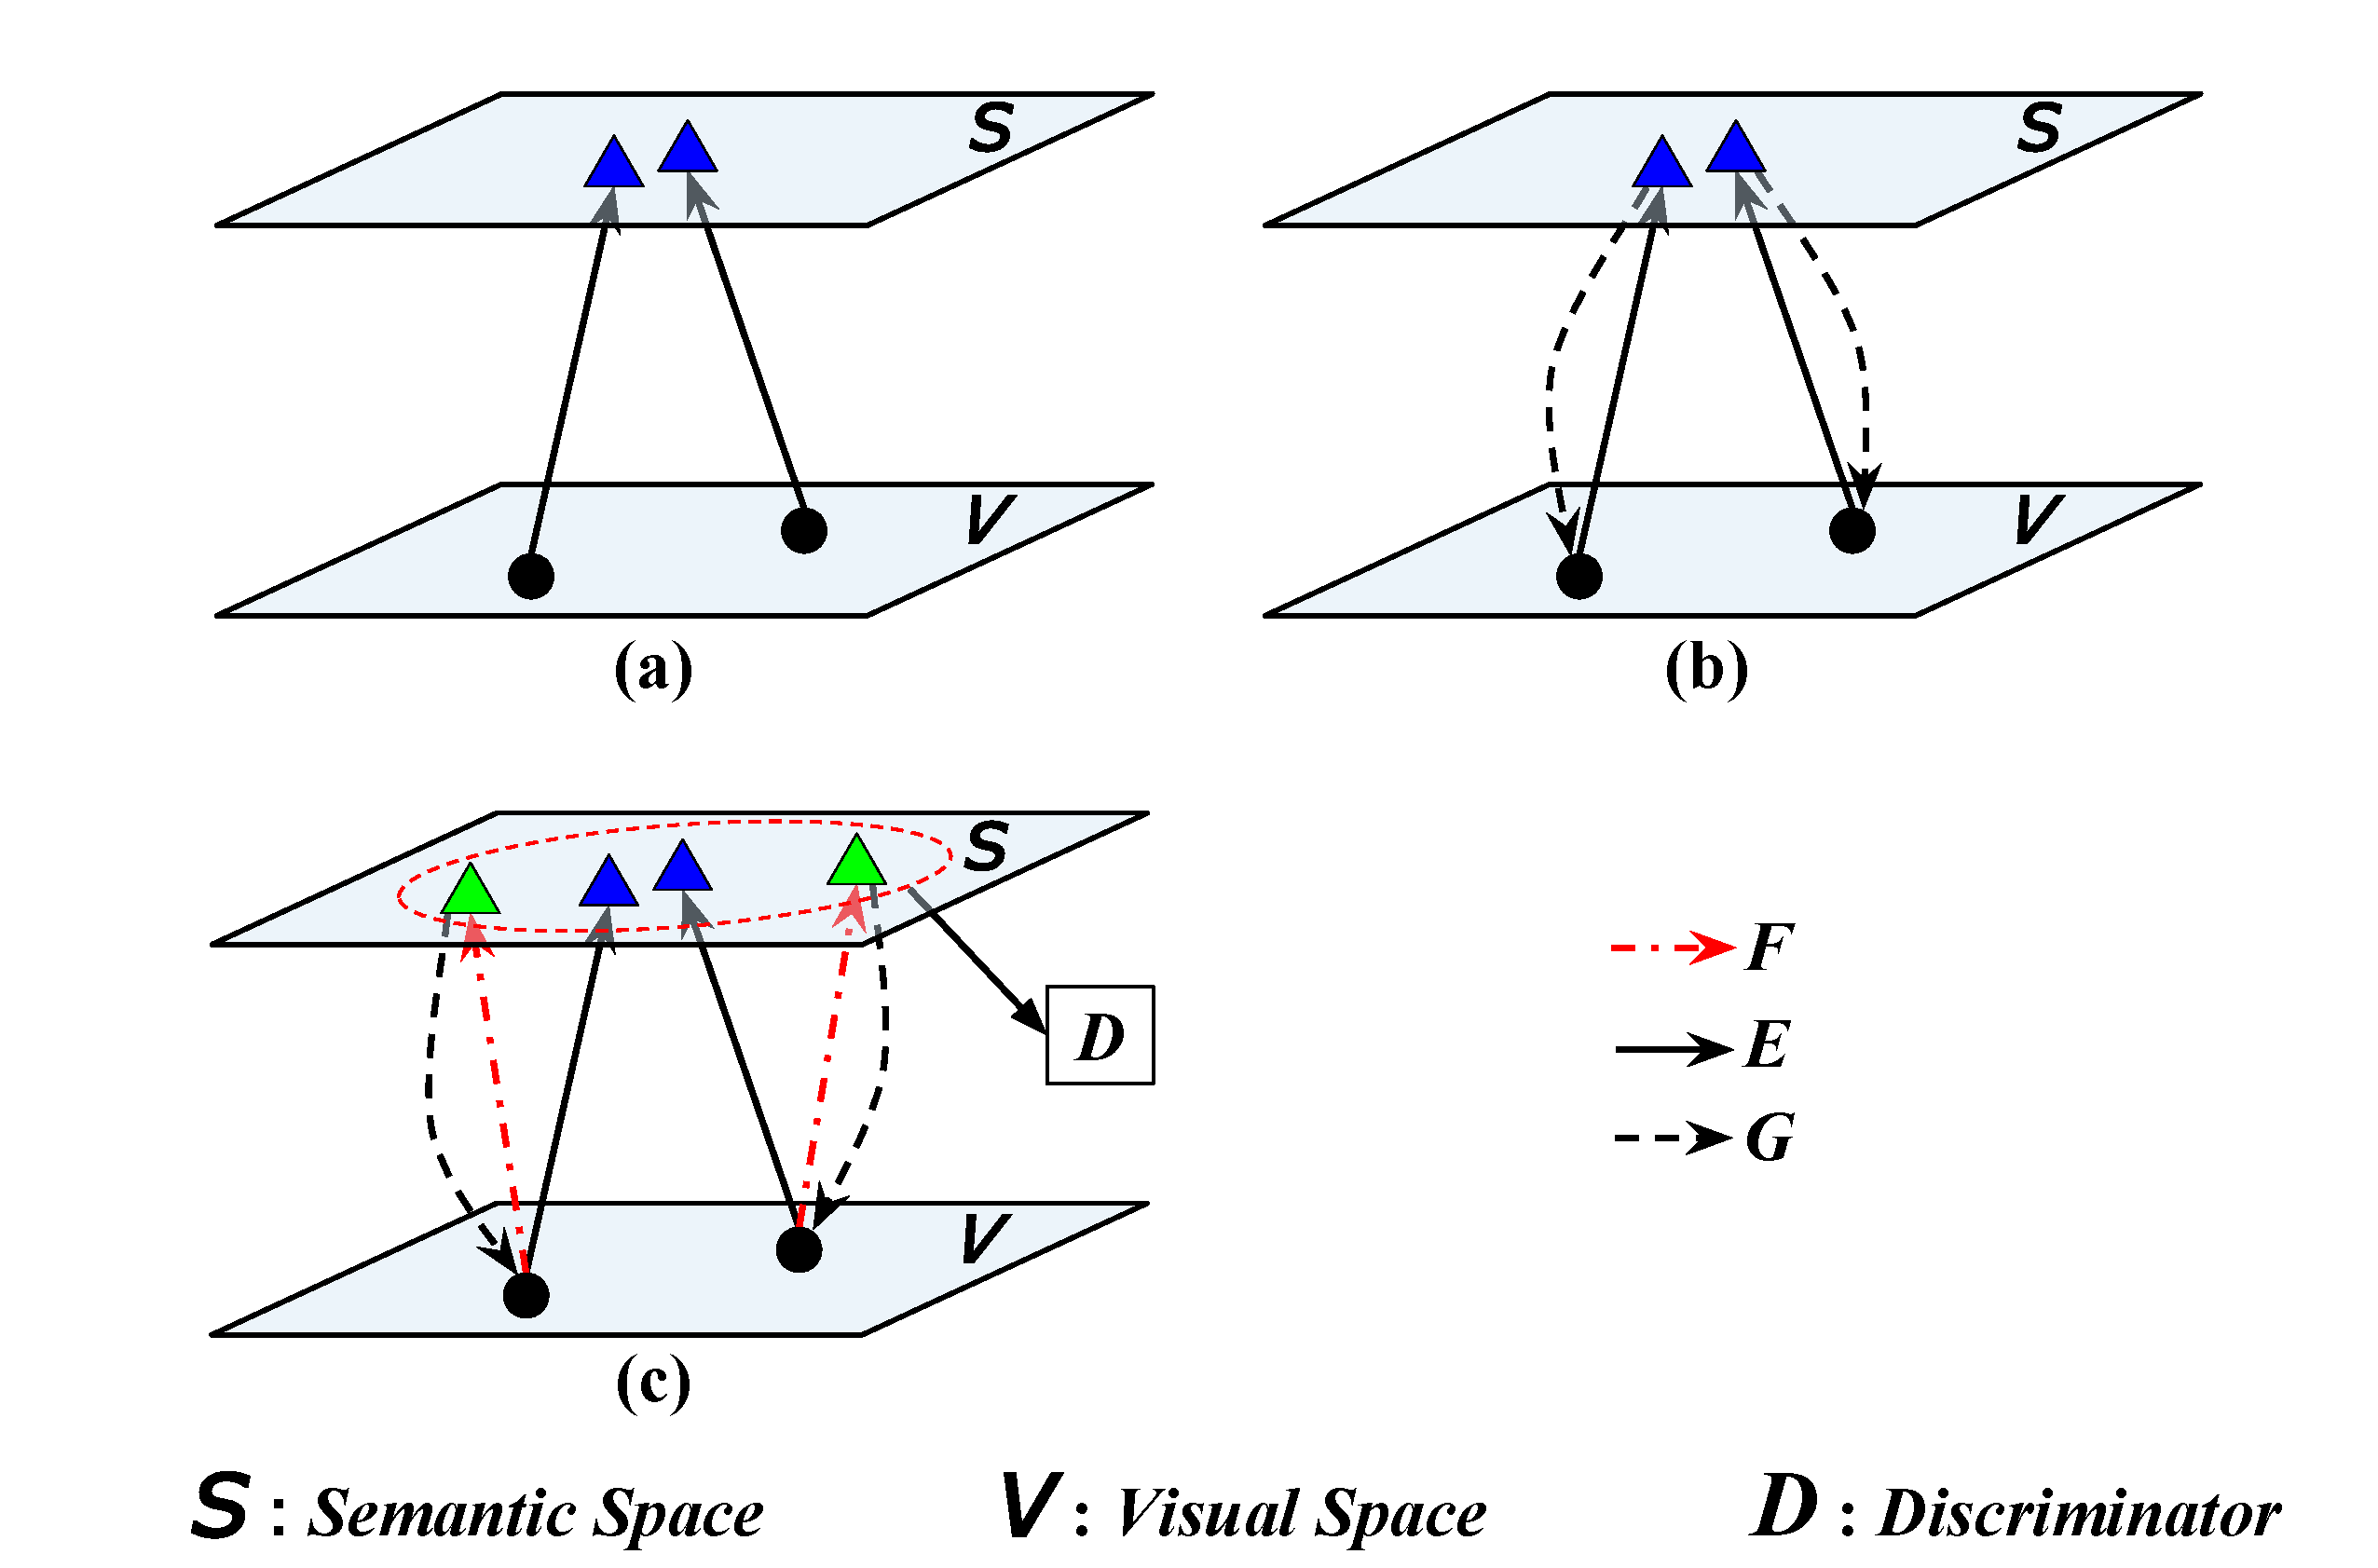
\includegraphics[width=0.98\linewidth]{chapter3/res/zsl_paradigms.pdf}
    \captionof{figure}{三种典型的零样本学习框架}
    \label{ch3:fig:zsl_paradigms}
\end{wrapfigure}

然而,这种嵌入映射模型的知识迁移能力受限于\textbf{语义丢失}的问题。如图~\ref{ch3:fig:zsl_paradigms}所示,模型在训练过程中往往丢失一些对训练集图像方差较小的属性(即,不同类别之间区别小的属性),这样有利于训练集的分类。然而,由于训练集和测试集之间的类别存在差异,这些丢失的属性可能对测试集的类别图像来说具有较明显的区别性,进而就会增加测试集分类的困难。虽然每个类别在语义空间$\mathcal{S}$中都只是一个单独的“点”,能够具有丰富的语义信息,但是将所有同类的图像从视觉空间$\mathcal{V}$映射到这个点附近,就不可避免地造成部分属性的丢失~\cite{lazaridou2015hubness,fu2015transductive}。


为了尽可能多地减少训练过程中属性的丢失,一个可能的解决方法是通过图像重建,即先将图像从视觉空间映射到语义空间中,然后将语义空间的特征映射回视觉空间。如果映射回视觉空间的特征能够重建初始的图像,说明语义空间的特征已经尽可能多地保持了原有的属性,否则图像将无法重建~\cite{kim2017learning,yi2017dualgan,zhu2017unpaired,he2016dual}。然而,图像重建和图像分类是两个相互冲突的目标:前者希望能够尽可能多地保持图像的细节,而后者希望只关注类别差异性大的特征,忽略不相关的特征。例如,只用“头”或者“躯干”就可以充分地对“人”这个类别进行识别分类,而一些其他的颜色属性,如“红色”或者“白色”就需要忽略。为了进一步展示重建和分类这两个冲突任务,如图~\ref{ch3:fig:zsl_paradigms}(b)所示,假设 $E$:$\mathcal{V}\rightarrow \mathcal{S}$和$G$:$\mathcal{S}\rightarrow \mathcal{V}$是视觉空间$\mathcal{V}$与语义空间$\mathcal{S}$中的两个映射函数。对于图像分类任务,我们希望视觉空间中同一类别的两个图像$x, x'\in \mathcal{V}$在语义空间能够接近$s, s'\in\mathcal{S}$, 即$E(x) = s \approx s' = E(x')$;对于图像重建任务,我们希望$G(s)\approx x$和$G(s')\approx x'$,这样就很难满足$s\approx s'$。因此,同时训练图像分类和图像重建两个目标,对于保持属性的效果往往有限(如模型SAE~\cite{kodirov2017semantic})。如图~\ref{ch3:fig:reconstruction_visualization}所示,当我们想实现好的图像分类结果时,图像重建往往会失败。

\begin{figure}[h]
    \centering
        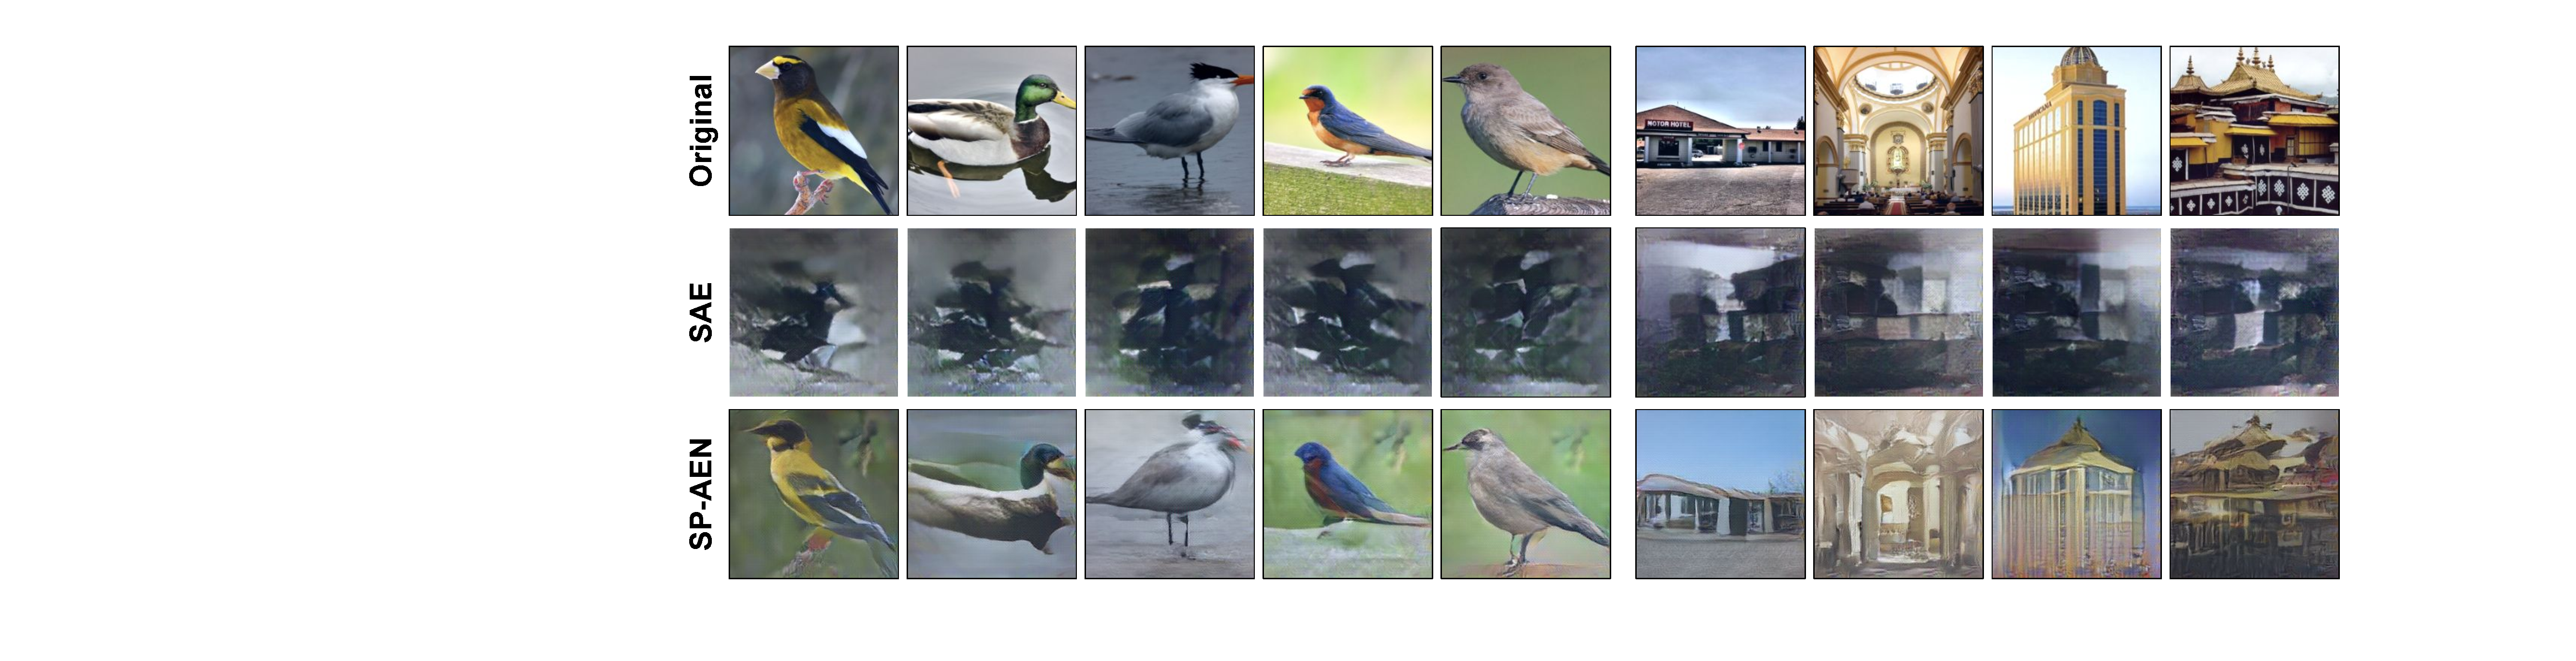
\includegraphics[width=\linewidth]{chapter3/res/reconstruction_visualization.pdf}
    \caption{模型SAE和模型SP-AEN的图像重建结果对比}
    \label{ch3:fig:reconstruction_visualization}
\end{figure}

为了缓解图像分类任务和图像重建任务之间的冲突,本文提出一个全新的零样本物体分类网络:属性保持对抗网络(SP-AEN)。如图~\ref{ch3:fig:zsl_paradigms}(c)所示,我们引入一个新的映射函数$F$:$\mathcal{V}\rightarrow \mathcal{S}$和一个对抗优化目标~\cite{goodfellow2014generative}。映射函数$F$和对抗训练的目的是让判别器$D$无法区分这两个不同的映射分布$E(x)$和$F(x)$。具体来说,这样做有两个好处:(1)语义迁移:虽然对于单独的分类映射函数$E$来说,语义丢失问题是不可避免的。但是,我们通过利用判别器$D$的训练,让分类映射向量$E(x)$和重建映射向量$F(x)$在同一个分布下,实现属性特征的迁移,让$E(x)$尽可能地保持更多的属性。(2)分类任务与重建任务分解:映射网络$F$和$G$实现重建任务,而映射网络$E$实现分类任务。通过将分类任务和重建任务进行分解,之前的严格条件$G(E(x)) \approx x$和$G(E(x')) \approx x'$变成了$G(F(x))\approx x$和$G(F(x'))\approx x'$,同时$F(x)$与$F(x')$在语义空间中也不需要非常接近。如图~\ref{ch3:fig:reconstruction_visualization}所示,我们的映射$G(F(x))$可以重建出较好的输入图像,说明属性特征能够更好地保持。

本文在零样本分类任务通用的四个数据集CUB~\cite{wah2011caltech}、AWA~\cite{lampert2009learning}、SUN~\cite{patterson2012sun}和aPY~\cite{farhadi2009describing}中对模型SP-AEN的效果进行验证。相比于目前性能最好的零样本分类方法~\cite{xian2017zero},SP-AEN在评价指标H值(harmonic mean value)上对于上述四个数据集分别提升了12.2\%、9.3\%、4.0\%和3.6\%。同时,SP-AEN是第一个能够直接重建回原始图像的零样本分类模型。


\section{属性保持对抗网络}

在本节,我们首先介绍零样本分类任务,然后再具体介绍本章提出模型SP-AEN的各个优化目标的细节。

\subsection{零样本分类预备知识}
给定一个训练集$\{x_i, l_i\}$,其中$x_i\in\mathcal{V}$是图像在视觉空间的映射向量,$l_i\in \mathcal{L}_s$是已见类别的类别标签。零样本物体分类任务的目标是学习一个分类器,不仅可以预测已见类别的图像($\mathcal{L}_s$),也可以预测未见类别的图像($\mathcal{L}_u$)。按照之前零样本物体分类方法的总结~\cite{xian2017zero,lei2015predicting},几乎所有先进的零样本分类方法都是基于嵌入映射框架的。这类方法旨在找到一个映射函数$E$:$\mathcal{V}\rightarrow \mathcal{S}$,其中所有的类别标签在语义空间$\mathcal{S}$都是编码成$\bm{y}_l\in\mathbb{R}^d$。因此,预测类别标签$l^*$时,可以直接通过简单的最近邻查找得到:
\begin{equation}\label{ch3:eq:eq_1}
l^* = \max_{l\in\mathcal{L}}~\bm{y}^T_l E(x)
\end{equation}
特别地,如果$l\in\mathcal{L}_u$,这类零样本分类问题称为\textbf{传统型零样本分类}(conventional ZSL);如果$l \in\mathcal{L}_s\cup \mathcal{L}_u$,这类零样本分类问题称为\textbf{通用型零样本分类}(generalized ZSL)。另外,公式~\eqref{ch3:eq:eq_1}中映射函数$E$即可以是线性函数,也可以是基于深度神经网络的非线性函数。


\begin{figure}[tbp]
    \centering
        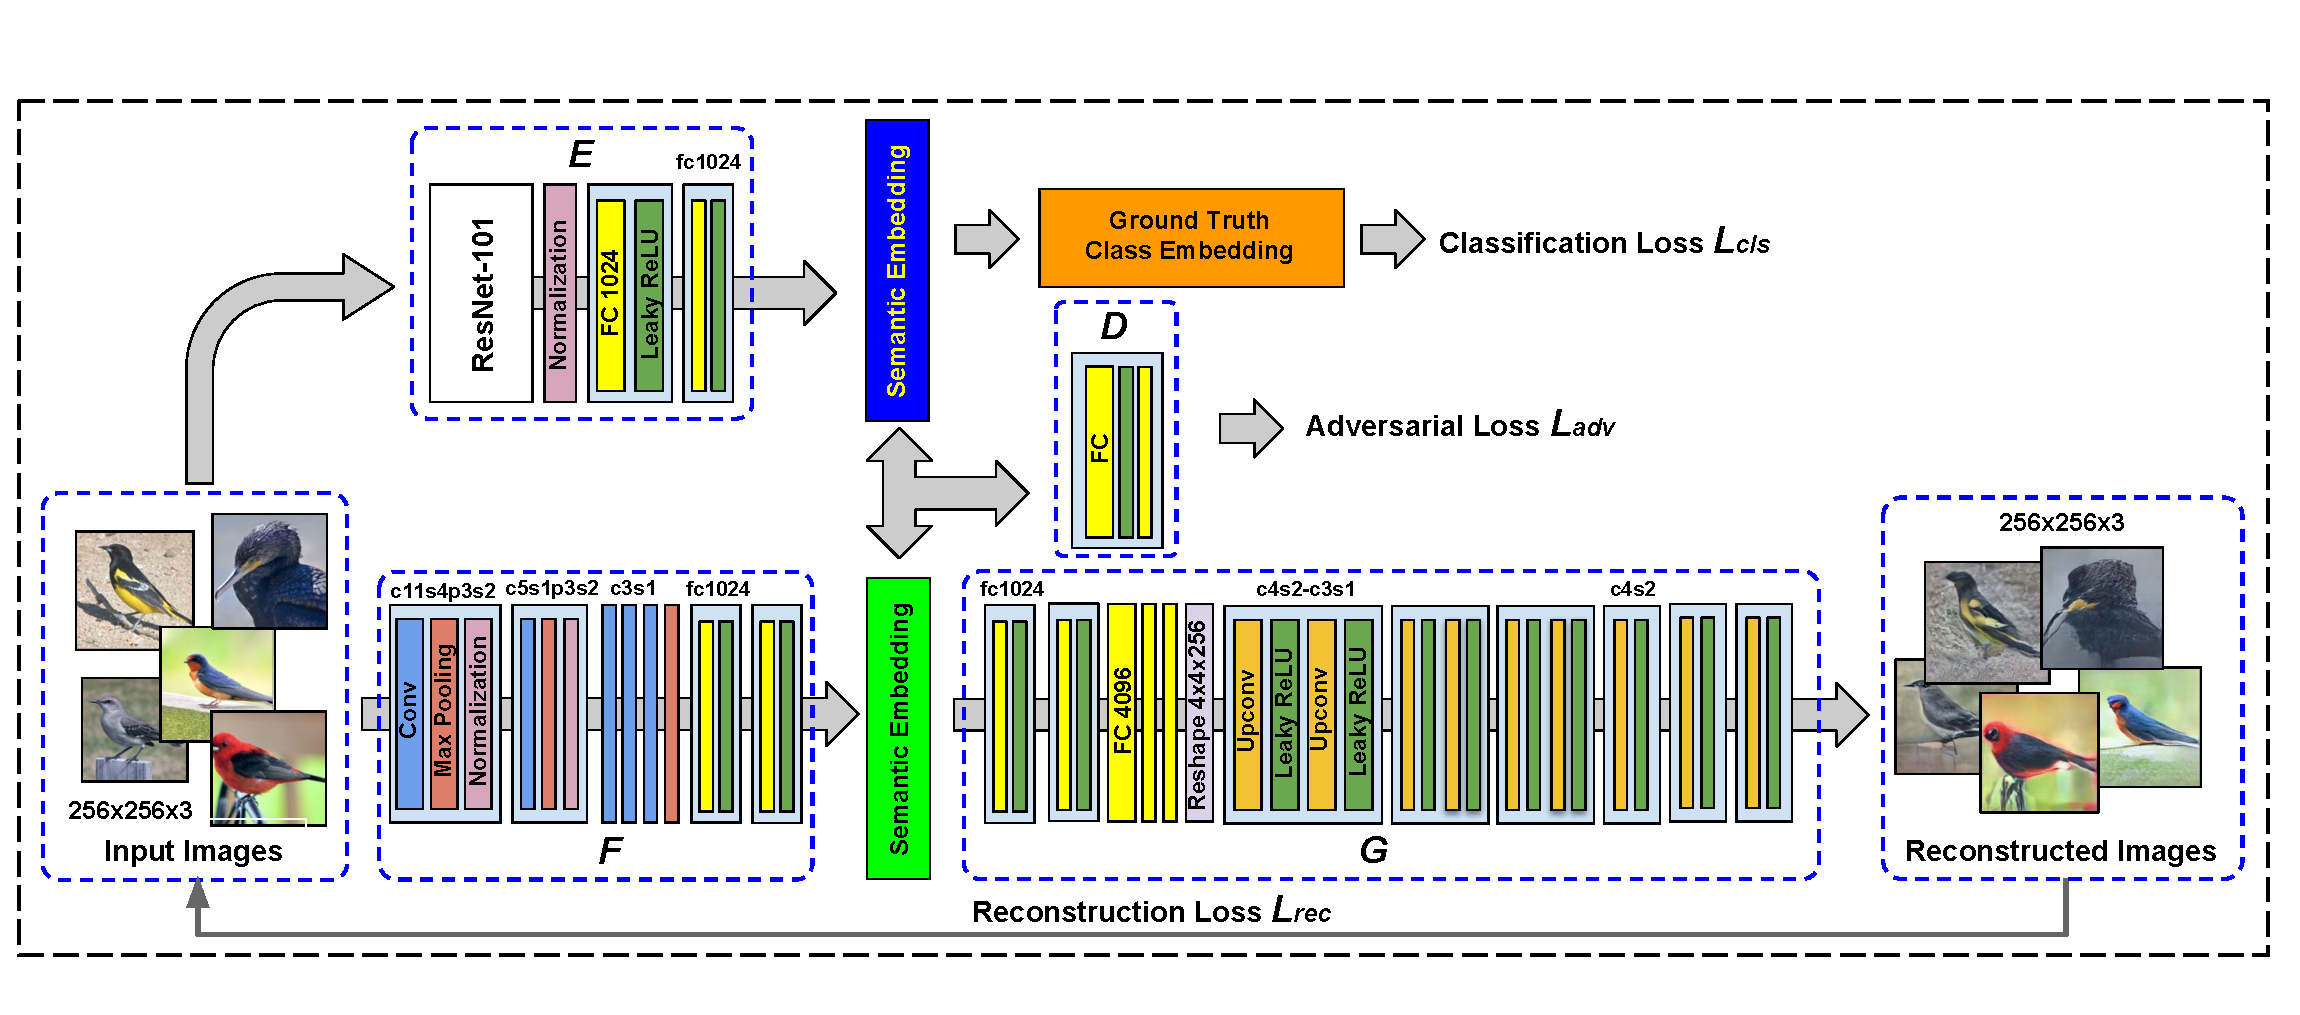
\includegraphics[width=\linewidth]{chapter3/res/sp_aen.pdf}
    \caption{模型SP-AEN的整体网络结构流程图}
    \label{ch3:fig:sp_aen}
\end{figure}


\subsection{分类任务优化目标}
因为公式~\eqref{ch3:eq:eq_1}的类别预测问题本质上是一个排序问题,所以我们直接使用排序损失函数(ranking loss)作为分类任务的优化目标~\cite{frome2013devise,weston2010large}。具体来说,给定一个训练样本$(x, l)$,我们希望$\bm{y}_l$和$E(x)$之间的点积相似度较大;而对于负样本$(x,l')$,$\bm{y}_{l'}$和$E(x)$之间的点积相似度较小;同时正样本的相似度相比负样本的相似度要大于一定的阈值$\gamma$:
\begin{equation} \label{ch3:eq:eq_2}
L_{cls} = \sum\limits_{l\neq l'}~\max\{0, \gamma - \bm{y}_l^T E(x) + \bm{y}^T_{l'} E(x)\}
\end{equation}
其中,阈值$\gamma$是一个大于0的超参数。在每次训练迭代过程中,$l'$是从所有错误的类别标签中随机任选的一个。

分类任务的优化目标$L_{cls}$主要是让所有的同一类图像的语义空间映射向量$E(x)$都接近与其类别标签在语义空间的映射向量$\bm{y}$。它造成的语义丢失问题将由后续介绍的两个优化目标(重建任务优化目标和对抗学习优化目标)来解决。


\subsection{重建任务优化目标}
重建任务的目标是学习一个从语义空间到视觉空间的映射函数$G$:$\mathcal{S}\rightarrow \mathcal{V}$,使得将语义映射向量$s\in\mathcal{S}$可以重建出输入图像,并且使差别$\|G(s)-x\|$很小。由于在自编码器形式的网络中重建任务$s = E(x)$与分类任务是相互冲突的,我们引入一个新的视觉空间到语义空间的映射函数$F$,使得$s = F(x)$。另外,不同于SAE~\cite{kodirov2017semantic}利用卷积神经网络~\cite{he2016deep,simonyan2015very}的高层输出向量作为视觉空间$\mathcal{V}$的特征,我们直接利用原始的$256\times 256 \times 3$大小的RGB色彩空间来进行图像重建。这样做的主要原因是卷积神经网络的输出特征在网络的预训练阶段已经存在语义丢失。


为了最小化重建损失,映射向量$F(x)$会尽可能地保持多的属性,以便于能够重建回原始输入图像。我们参考最新的图像生成工作~\cite{johnson2016perceptual,dosovitskiy2016generating,ledig2017photo},将重建任务的优化目标定义为:
\begin{equation}\label{ch3:eq:eq_3}
L_{rec} = L_{feat}+\lambda_p L_{pixel}
\end{equation}
其中$L_{feat} = \|\phi\left(G\left(F(x)\right)\right)-\phi(x)\|^2_2$是特征空间上的重建损失函数,帮助图像能够保持细节感知上的相似度。我们使用卷积神经网络AlexNet~\cite{krizhevsky2012imagenet}中conv5层来表示函数$\phi$。$L_{pixel} = \|G(F(x))-x\|^2_2$是像素空间上的重建损失函数,有利于重建算法训练过程的稳定性。


\subsection{对抗学习优化目标}
到目前为止,语义向量$E(x)$和$F(x)$之间还没有进行知识迁移。我们的目标是让$E(x)$从$F(x)$中迁移部分丢失的属性特征。因为手工直接定义$E(x)$与$F(x)$之间的迁移方式比较困难,所以我们借助对抗学习的思想,来鼓励$E(x)$的分布向$F(x)$的分布靠近,通过“欺骗”判别网络$D$,来实现$F(x)$的知识向$E(x)$迁移:
\begin{equation} \label{ch3:eq:eq_4}
L_{adv} = \mathbb{E}_{x}\left( \log D(F(x)) \right) + \mathbb{E}_{x'}\left( \log \left[1-D(E(x'))\right] \right)
\end{equation}
其中网络$E$为了减少优化目标$L_{adv}$,而网络$D$希望增大优化目标$L_{adv}$,即:$E^* = \arg\min_E \max_D L_{adv}$。

目前,许多研究工作都发现目标函数$L_{adv}$的优化过程容易导致塌陷问题~\cite{arjovsky2017wasserstein}(mode collapse)。在零样本物体分类任务中,如果两个同类别的两个图像$x$和$x'$非常相似,同样容易导致$\|F(x)-E(x')\|\approx 0$,引起塌陷问题。为了避免塌陷问题,我们参考WGAN~\cite{arjovsky2017wasserstein}的训练策略,极大地增加了模型训练的稳定性。


\subsection{总体优化目标}
将前文提到的分类任务优化目标、重建任务优化目标、以及对抗学习优化目标合在一起,得到模型SP-AEN最终整体的优化目标:
\begin{equation} \label{ch3:eq:eq_5}
L (E, F, G, D) = L_{cls}(E) + \alpha L_{rec} (E, F, G) + \beta L_{adv}(E, F, G, D)
\end{equation}
其中,$\alpha$和$\beta$是超参数用于权衡不同的优化目标函数的权重。我们最终的目标是得到:
\begin{equation}\label{ch3:eq:eq_6}
E^* = \arg\min\limits_{E, F, G}\max\limits_{D} L(E, F, G, D)
\end{equation}

如图~\ref{ch3:fig:sp_aen}所示,网络$F$是重建任务编码网络,网络$G$是重建任务解码网络,重建任务映射向量$F(x)$可以看成是瓶颈层,来约束分类任务映射向量$E(x)$。另外,模型SP-AEN也可以无缝地运用到其他实验设定下的零样本物体分类问题,例如在半监督条件下,我们只需要给$F(x)$增加一个额外的对抗学习优化目标来近似先验的映射空间。


\section{实验设置与性能分析}
\subsection{零样本物体分类数据集}

我们在四个通用的零样本物体分类数据集(CUB、SUN、AWA、aPY)上对模型SP-AEN的性能进行了验证。其中,我们参考Xian等人~\cite{xian2017zero}使用新的数据集划分。因为之前的零样本分类工作都使用ILSVRC ImageNet~\cite{russakovsky2015imagenet}上的1000个常见类图像对卷积神经网络进行预训练,而这1000类与这四个数据集的原始划分都有重叠类别,即违背了零样本物体分类的基本设定。以下是这四个数据集的详细介绍:

\textbf{CUB}~\cite{wah2011caltech}:全称是Caltech-UCSD-Birds 200-2011数据集。它是一个细粒度鸟类别数据集,总共包含11788张来自200个细粒度类别的鸟图像,并且每张图像标注了312个语义属性。在通用型零样本分类的实验设定中,训练集包含150个已见类别的7057张图像,测试集包含150个已见类别的1764张图像和50个未见类别的2967张图像。

\textbf{SUN}~\cite{patterson2012sun}:全称是SUN attribute数据集。它是一个细粒度场景分类数据集,总共包含14340张来自717个场景类别的场景图像,并且每张图像标注了102个语义属性。在通用型零样本分类的实验设定中,训练集包含645个已见类别的10320张图像,测试集包含645个已见类别的2580张图像和72个未见类别的1440张图像。

\textbf{AWA}~\cite{lampert2009learning}:全称是Animals with Attributes数据集。它是一个动物类别分类数据集,总共包含30475张来自50个类别的动物图像,并且每张图像标注了85个语义属性。在通用型零样本分类的实验设定中,训练集包含40个已见类别的23527张图像,测试集包含40个已见类别的5882张图像和10个未见类别的7913张图像。由于原始AWA数据集图像版权的问题,我们这里的AWA数据集实际上使用的是AWA2~\cite{xian2017zero,xian2018zero}。

\textbf{aPY}~\cite{farhadi2009describing}:全称是Attribute Pascal and Yahoo数据集。它是一个通用的物体分类数据集,总共包含12051张来自32个类别,并且每张图像标注了64个语义属性。在通用型零样本分类的实验设定中,训练集包含20个已见类别5932张图像,测试集包含20个已见类别1483张图像和12个未见类别的7924张图像。

为了公平地和其他零样本物体分类模型进行比较,我们参考Xian等人~\cite{xian2017zero}使用完全相同的类别嵌入映射向量,并对所有的嵌入映射向量进行$l_2$范数归一化。


\subsection{实验设定与零样本物体分类评价指标}
\textbf{\kaishu{实验设定}}:为了充分地评估模型SP-AEN的零样本物体分类性能,我们在三种不同的实验设定下进行对比:
\begin{asparaenum}
\item U$\to$U:测试图像的类别和预测的类别标签都只限于未见类别;

\item S$\to$T:测试图像的类别只限于未见类别,但预测的类别标签可以是未见类别或已见类别;

\item U$\to$T:测试图像的类别和预测的类别标签都可以是未见类别或已见类别。
\end{asparaenum}
通常,U$\to$U被称为传统型零样本分类,而U$\to$T被称为通用型零样本分类。

\textbf{\kaishu{评价指标}}:我们参考之前的工作~\cite{xian2017zero},使用每个类别的平均准确率作为三个实验设定下的评价指标(即:$Acc_{U\rightarrow U}$、$Acc_{S\rightarrow T}$和$Acc_{U\rightarrow T}$)。对于通用型零样本分类,我们另外使用常用的$H$值作为主要的评价指标,其中$H$值是已见类别的准确率$Acc_{S\rightarrow T}$和未见类别的准确率$Acc_{U\rightarrow T}$的调和平均数:
\begin{equation} \label{ch3:eq:eq_7}
H = 2\times Acc_{S\rightarrow T}\times Acc_{U\rightarrow T} /(Acc_{S\rightarrow T}+Acc_{U\rightarrow T})
\end{equation}

\subsection{网络模型与训练细节}
\textbf{\kaishu{网络结构}}:整个模型SP-AEN的网络结构如图~\ref{ch3:fig:sp_aen}所示。其中分类映射网络$E$是基于网络ResNet-101~\cite{he2016deep}。网络$E$的输入是大小为$224\times224\times3$的原始图像,输出是$d$维的编码向量,然后输入到分类优化函数中(即公式~\eqref{ch3:eq:eq_2})。重建编码网络$F$是基于网络AlexNet~\cite{krizhevsky2012imagenet},并加上两层额外的全连接层。和分类网络$E$类似,输入是$224\times224\times3$的原始图像,输出是$d$维的编码向量。但是,输出的编码向量再输给重建解码网络$G$。重建解码网络$G$通过五个连续的反卷积和非线性激活函数(leaky ReLU~\cite{he2015delving})将向量转换成三维特征图。另外,在重建解码网络的头部我们使用两个全连接层先将编码向量的维度映射到4096维。判别器网络$D$是一个两层的全连接层加一个非线性ReLU层,网络$D$的输入为$d$维的编码向量。

\textbf{\kaishu{训练细节}}:对于本章所有的零样本分类实验,我们都先将训练图像的短边放缩到256,然后参照AlexNet~\cite{krizhevsky2012imagenet}数据增强的策略增大十倍训练数据。为了提升训练速度,分类映射网络$E$中ResNet-101采用ImageNet数据集上预训练好的ResNet-101的参数,并始终固定参数。重建编码网络$F$的参数初始化采用ImageNet数据集上预训练好的AlexNet的参数,重建解码网络$G$采用预训练好的生成器~\cite{dosovitskiy2016generating}作初始化。剩余网络中的所有参数都采用MSRA初始化~\cite{he2015delving}。初始的学习率设置为$1e^{-4}$,训练过程中当损失函数不再下降时,学习率降低10倍继续训练。


\subsection{零样本物体分类的性能对比}
本节将本章提出的模型SP-AEN与目前最先进的零样本物体分类方法进行对比。这些方法主要可以分类:(1)基于嵌入映射的模型:\textbf{DeViSE}~\cite{frome2013devise}、\textbf{ALE}~\cite{akata2015label}、\textbf{SJE}~\cite{akata2015evaluation}、\textbf{ESZSL}~\cite{romera2015embarrassingly}、\textbf{LTM}\cite{xian2016latent}、\textbf{CMT}~\cite{socher2013zero}和\textbf{SAE}~\cite{kodirov2017semantic}。这类方法和SP-AEN一样,都是将图像从视觉空间映射到语义空间,其中SAE是目前现有的唯一一个利用信号重建来解决语义损失的模型。(2)基于属性的模型:\textbf{DAP}~\cite{lampert2009learning}、\textbf{IAP}~\cite{lampert2009learning}、\textbf{SSE}~\cite{zhang2015zero}、\textbf{CSE}~\cite{norouzi2014zero}和\textbf{SYNC}~\cite{changpinyo2016synthesized}。特别地,这类方法只适用于所有类别都有人工标注属性的情况下。

%%%%%%%%%%%%%%%%%%%%%%%%%% SOTA %%%%%%%%%%%%%%%%%%%%
\begin{table}[htbp]
\centering
\scalebox{0.7}{
\begin{tabular}{|c | c | c c c c c c c c c c c c c|}
\hline
Dataset &  & DAP & IAP & SSE & CSE & SYNC & CMT & LTM & DeViSE & ALE & SJE & ESZSL & SAE & SP-AEN \\
\hline
\multirow{4}{*}{SUN} & $Acc_{U\to U}$ & 39.9 & 19.4 & 51.5 & 38.8 & 56.3 & 39.9 & 55.3 & 56.5 & 58.1 & 53.7 & 54.5 & 40.3 & \textbf{59.2} \\
& $Acc_{U\to T}$ & 4.2 & 1.0 & 2.1 & 6.8 & 7.9 & 8.1 & 14.7 & 16.9 & 21.8 & 14.7 & 11.0 & 8.8 & \textbf{24.9} \\
& $Acc_{S\to T}$ & 25.1 & 37.8 & 36.4 & \textbf{39.9} & 43.3 & 21.8  & 28.8 & 27.4 & 33.1 & 30.5 & 27.9 & 18.0 & 38.6 \\
\rowcolor[gray]{0.9}
& H & 7.2 & 1.8 & 4.0 & 11.6 & 13.4 & 11.8 & 19.5 & 20.9 & 26.3 & 19.8 & 15.8 & 11.8 & \textbf{30.3} \\
\hline
\multirow{4}{*}{CUB} & $Acc_{U\to U}$ & 40.0 & 24.0 & 43.9 & 34.3 & \textbf{55.6} & 34.6 & 49.3 & 52.0 & 54.9 & 53.9 & 53.9 & 33.3 & 55.4 \\
& $Acc_{U\to T}$ & 1.7 & 0.2 & 8.5 & 1.6 & 11.5 & 7.2 & 15.2 & 23.8 & 23.7 & 23.5 & 12.6 & 7.8 & \textbf{34.7} \\
& $Acc_{S\to T}$ & 67.9 & \textbf{72.8} & 46.9 & 72.2 & 70.9 & 49.8 & 57.3 & 53.0 & 62.8 & 59.2 & 63.8 & 54.0 & 70.6 \\
\rowcolor[gray]{0.9}
& H & 3.3 & 0.4 & 14.4 & 3.1 & 19.8 & 12.6 & 24.0 & 32.8 & 34.4 & 33.6 & 21.0 & 13.6 & \textbf{46.6} \\
\hline
\multirow{4}{*}{AWA} & $Acc_{U\to U}$ & 46.1 & 35.9 & 61.0 & 44.5 & 46.6 & 37.9 & 55.8 & 59.7 & \textbf{62.5} & 61.9 & 58.6 & 54.1 & 58.5 \\
& $Acc_{U\to T}$ & 0.0 & 0.9 & 8.1 & 0.5 & 10.0 & 0.5 & 11.5 & 17.1 & 14.0 & 8.0 & 5.9 & 1.1 & \textbf{23.3} \\
& $Acc_{S\to T}$ & 84.7 & 87.6 & 82.5 & 90.6 & 90.5 & 90.0 & 77.3 & 74.7 & 81.8 & 73.9 & 77.8 & 82.2 & \textbf{90.9} \\
\rowcolor[gray]{0.9}
& H & 0.0 & 1.8 & 14.8 & 1.0 & 18.0 & 1.0 & 20.0 & 27.8 & 23.9 & 14.4 & 11.0 & 2.2 & \textbf{37.1} \\
\hline
\multirow{4}{*}{aPY} & $Acc_{U\to U}$ & 33.8 & 36.6 & 34.0 & 26.9 & 23.9 & 28.0 & 35.2 & \textbf{39.8} & 39.7 & 32.9 & 38.3 & 8.3 & 24.1 \\
& $Acc_{U\to T}$ & 4.8 & 5.7 & 0.2 & 0.0 & 7.4 & 1.4 & 0.1 & 4.9 & 4.6 & 3.7 & 2.4 & 0.4 & \textbf{13.7} \\
& $Acc_{S\to T}$ & 78.3 & 65.6 & 78.9 & \textbf{91.2} & 66.3 & 85.2 & 73.0 & 76.9 & 73.7 & 55.7 & 70.1 & 80.9 & 63.4 \\
\rowcolor[gray]{0.9}
& H & 9.0 & 10.4 & 0.4 & 0.0 & 13.3 & 2.8 & 0.2 & 9.2 & 8.7 & 6.9 & 4.6 & 0.9 & \textbf{22.6} \\
\hline
\end{tabular}
}
\caption{不同零样本分类模型在通用的四个零样本分类数据集上的性能对比}
\label{ch3:tab:sota}
\end{table}
%%%%%%%%%%%%%%%%%%%%%%%%%%%%%%%%%%%%%%%%%%%%%%%%%%%%%

\textbf{\kaishu{性能对比结果}}:表~\ref{ch3:tab:sota}总结了不同的零样本分类模型在数据集SUN、CUB、AWA和aPY)和三种不同实验设定(U$\to$U、U$\to$T和S$\to$T)下的性能对比。从表~\ref{ch3:tab:sota}的结果可以发现:(1)在通用型零样本分类中,SP-AEN能够显著提升实验性能。例如:在$Acc_{U\to T}$和H值两个指标下,SP-AEN能比目前最好的模型提升大约4\%到12\%。尤其当数据集中训练集和测试集所有属性方差的余弦相似度越大时(数据集SUN、CUB、AWA、aPY中,训练集和测试集所有属性方差的余弦相似度分别为0.9851、0.9575、0.7459、0.5847。),性能提升更加明显,这也从侧面反映模型SP-AEN可以有效地缓解语义丢失问题。(2)在传统型零样本分类中,在绝大多数的数据集中,SP-AEN同样可以得到最佳的性能。造成部分实验效果欠佳的主要原因可能是因为在U$\to$U的实验设定下,图像类别的搜索空间仅限于未见类别。然而,语义丢失可能导致未见类别的图像和已见类别非常接近,引起错误的预测。

\subsection{零样本物体分类方法分析}

\begin{table}[t]
\centering
\begin{tabular}{|c | c| c| c| c|}
\hline
Method & \textbf{SUN} & \textbf{CUB} & \textbf{AWA} & \textbf{aPY} \\
\hline
 DirectMap & 0.079 & 0.069 & 0.075 & 0.085 \\
 SAE & 0.285 & 0.281 & 0.259 &  0.275\\
SplitBranch & 0.070 & 0.058  & 0.059 & 0.076 \\
SP-AEN & \textbf{0.053}  & \textbf{0.040}& \textbf{0.047} & \textbf{0.055} \\
\hline
\end{tabular}
\caption{不同重建网络下重建图像与输入图像之间的平均像素差平方}
\label{ch3:tab:conflict_quantitative}
\end{table}

\textbf{\kaishu{分类任务与重建任务的冲突}}:为了验证本章提出模型SP-AEN的设计动机,即分类任务和重建任务是相互冲突的。我们设计了三种图像重建网络框架,如图~\ref{ch3:fig:conflict}所示,可以实现图像重建:(1)\textbf{DirectMap}:对于输入图像,我们首先使用网络$E$将图像从视觉空间映射到语义空间,得到语义嵌入向量,然后使用网络$G$将语义嵌入向量映射回视觉空间。在DirectMap中,我们固定网络$E$的参数(即预训练好的AlexNet网络参数),只训练网络$G$的参数。DirectMap模型可以衡量初始的语义嵌入向量能够包含多少语义信息。(2)\textbf{SAE}:我们采用与SAE模型~\cite{kodirov2017semantic}相同的框架,用重建网络$G$作为解码网络,分类网络$E$作为编码网络,并且利用其中的瓶颈层来进行分类任务。在训练过程中,我们同时更新网络$E$和网络$G$的参数。(3)\textbf{SplitBranch}:我们将网络$E$的输出分别输入到两个不同的支路网络中,并且对其中一条支路进行分类任务。然后将两条主路的输出合并到一起,并输入到网络$G$中进行重建。

\begin{wrapfigure}{r}{0.6\linewidth}
    \centering
        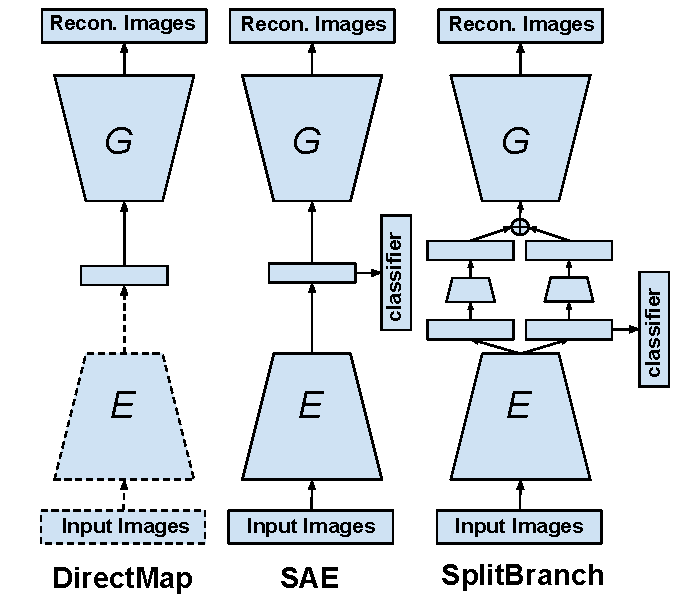
\includegraphics[width=0.95\linewidth]{chapter3/res/conflict.pdf}
    \captionof{figure}{三种不同的图像重建网络框架}
    \label{ch3:fig:conflict}
\end{wrapfigure}

图~\ref{ch3:fig:conflict_visualization}和表~\ref{ch3:tab:conflict_quantitative}分别表示四个数据集中测试集未见类别图像的重建图像和重建差异。从实验结果中,我们可以发现:(1)在数据集CUB和SUN中,DirectMap重建的图像和SP-AEN非常接近,都具有较好的重建结果。然而,在数据集AWA和aPY中,DirectMap的重建效果有明显下降。同样地,这是由于在数据集CUB和SUN中,训练集和测试集所有属性方差的余弦相似度较大,而数据集AWA和aPY中两者的余弦相似度较小。(2)对于SAE模型,当同时训练分类网络$E$和重建网络$G$时,所有的图像样本都重建失败。对于SplitBranch模型,当同时训练分类网络$E$和重建网络$G$时,重建效果得到显著的提升,接近模型SP-AEN。然而,在SplitBranch中,我们发现分类分支合并时的权重几乎为零。这一方面说明分类的映射向量基本对重建任务没有任何的贡献,另一方面这也引导我们借助对抗学习来实现语义迁移和高质量图像的重建。

\begin{figure}[t]
    \centering
    \scalebox{0.75}{
        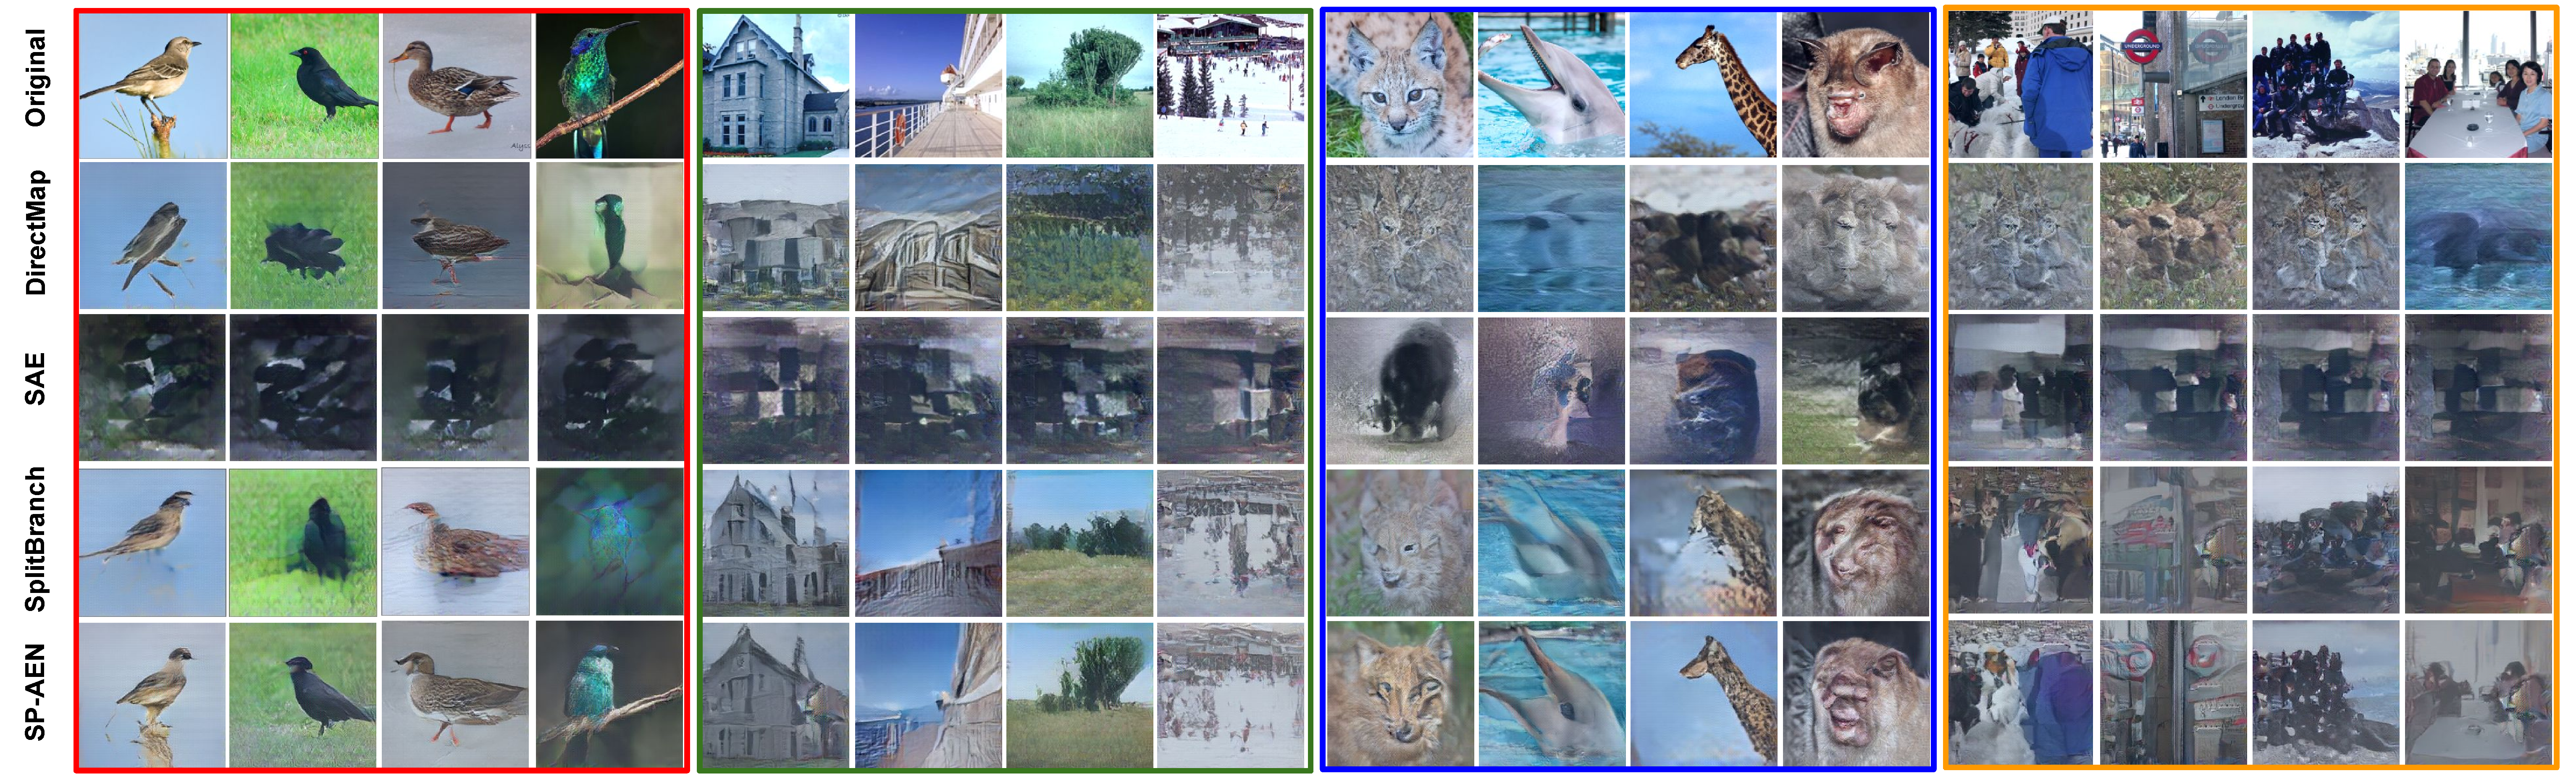
\includegraphics[width=\linewidth]{chapter3/res/conflict_visualization.pdf}    
    }
    \caption{不同图像重建网络框架在四个零样本物体分类数据集中的重建结果}
    \label{ch3:fig:conflict_visualization}
\end{figure}


\textbf{\kaishu{网络D和网络G的有效性}}:由于训练过程模型“见过”大量的已见类别图像,模型往往倾向于给已见类别赋予更高的分数。为了解决这个问题,通常使用“校准规则”(calibrated stacking rule)~\cite{chao2016empirical},即对已见类别的分数减掉一个常数偏置,然后再和未见类别的分数一起进行排序比较:
\begin{equation} \label{ch3:eq:eq_8}
    l^* = \max_{l\in \mathcal{L}_u \cup \mathcal{L}_s }~\bm{y}^T_l E(x) - \gamma \mathbf{1} \left[ l \in \mathcal{L}_s \right]
\end{equation}
其中指示函数$\mathbf{1} \left[ \cdot \right]$用于判断类别$l$是否是已见类别,$\gamma \in \mathbb{R}$是校准系数。这个校准规则能够有效地实现对已见类别和未见类别预测之间的权衡。通过不同调整校准系数$\gamma$,可以得到一系列分类准确率($Acc_{U \to T}$和$Acc_{S \to T}$)和已见-未见准确率曲线(Seen-Unseen accuracy Curve, SUC)。已见-未见准确率曲线下区域面积(Area Under Seen-Unseen accuracy Curve, AUSUC)也是通用型零样本分类问题中一个常用评价指标,用来评估$Acc_{U \to T}$和$Acc_{S \to T}$之间的权衡。

\begin{figure}[ht]
    \centering
    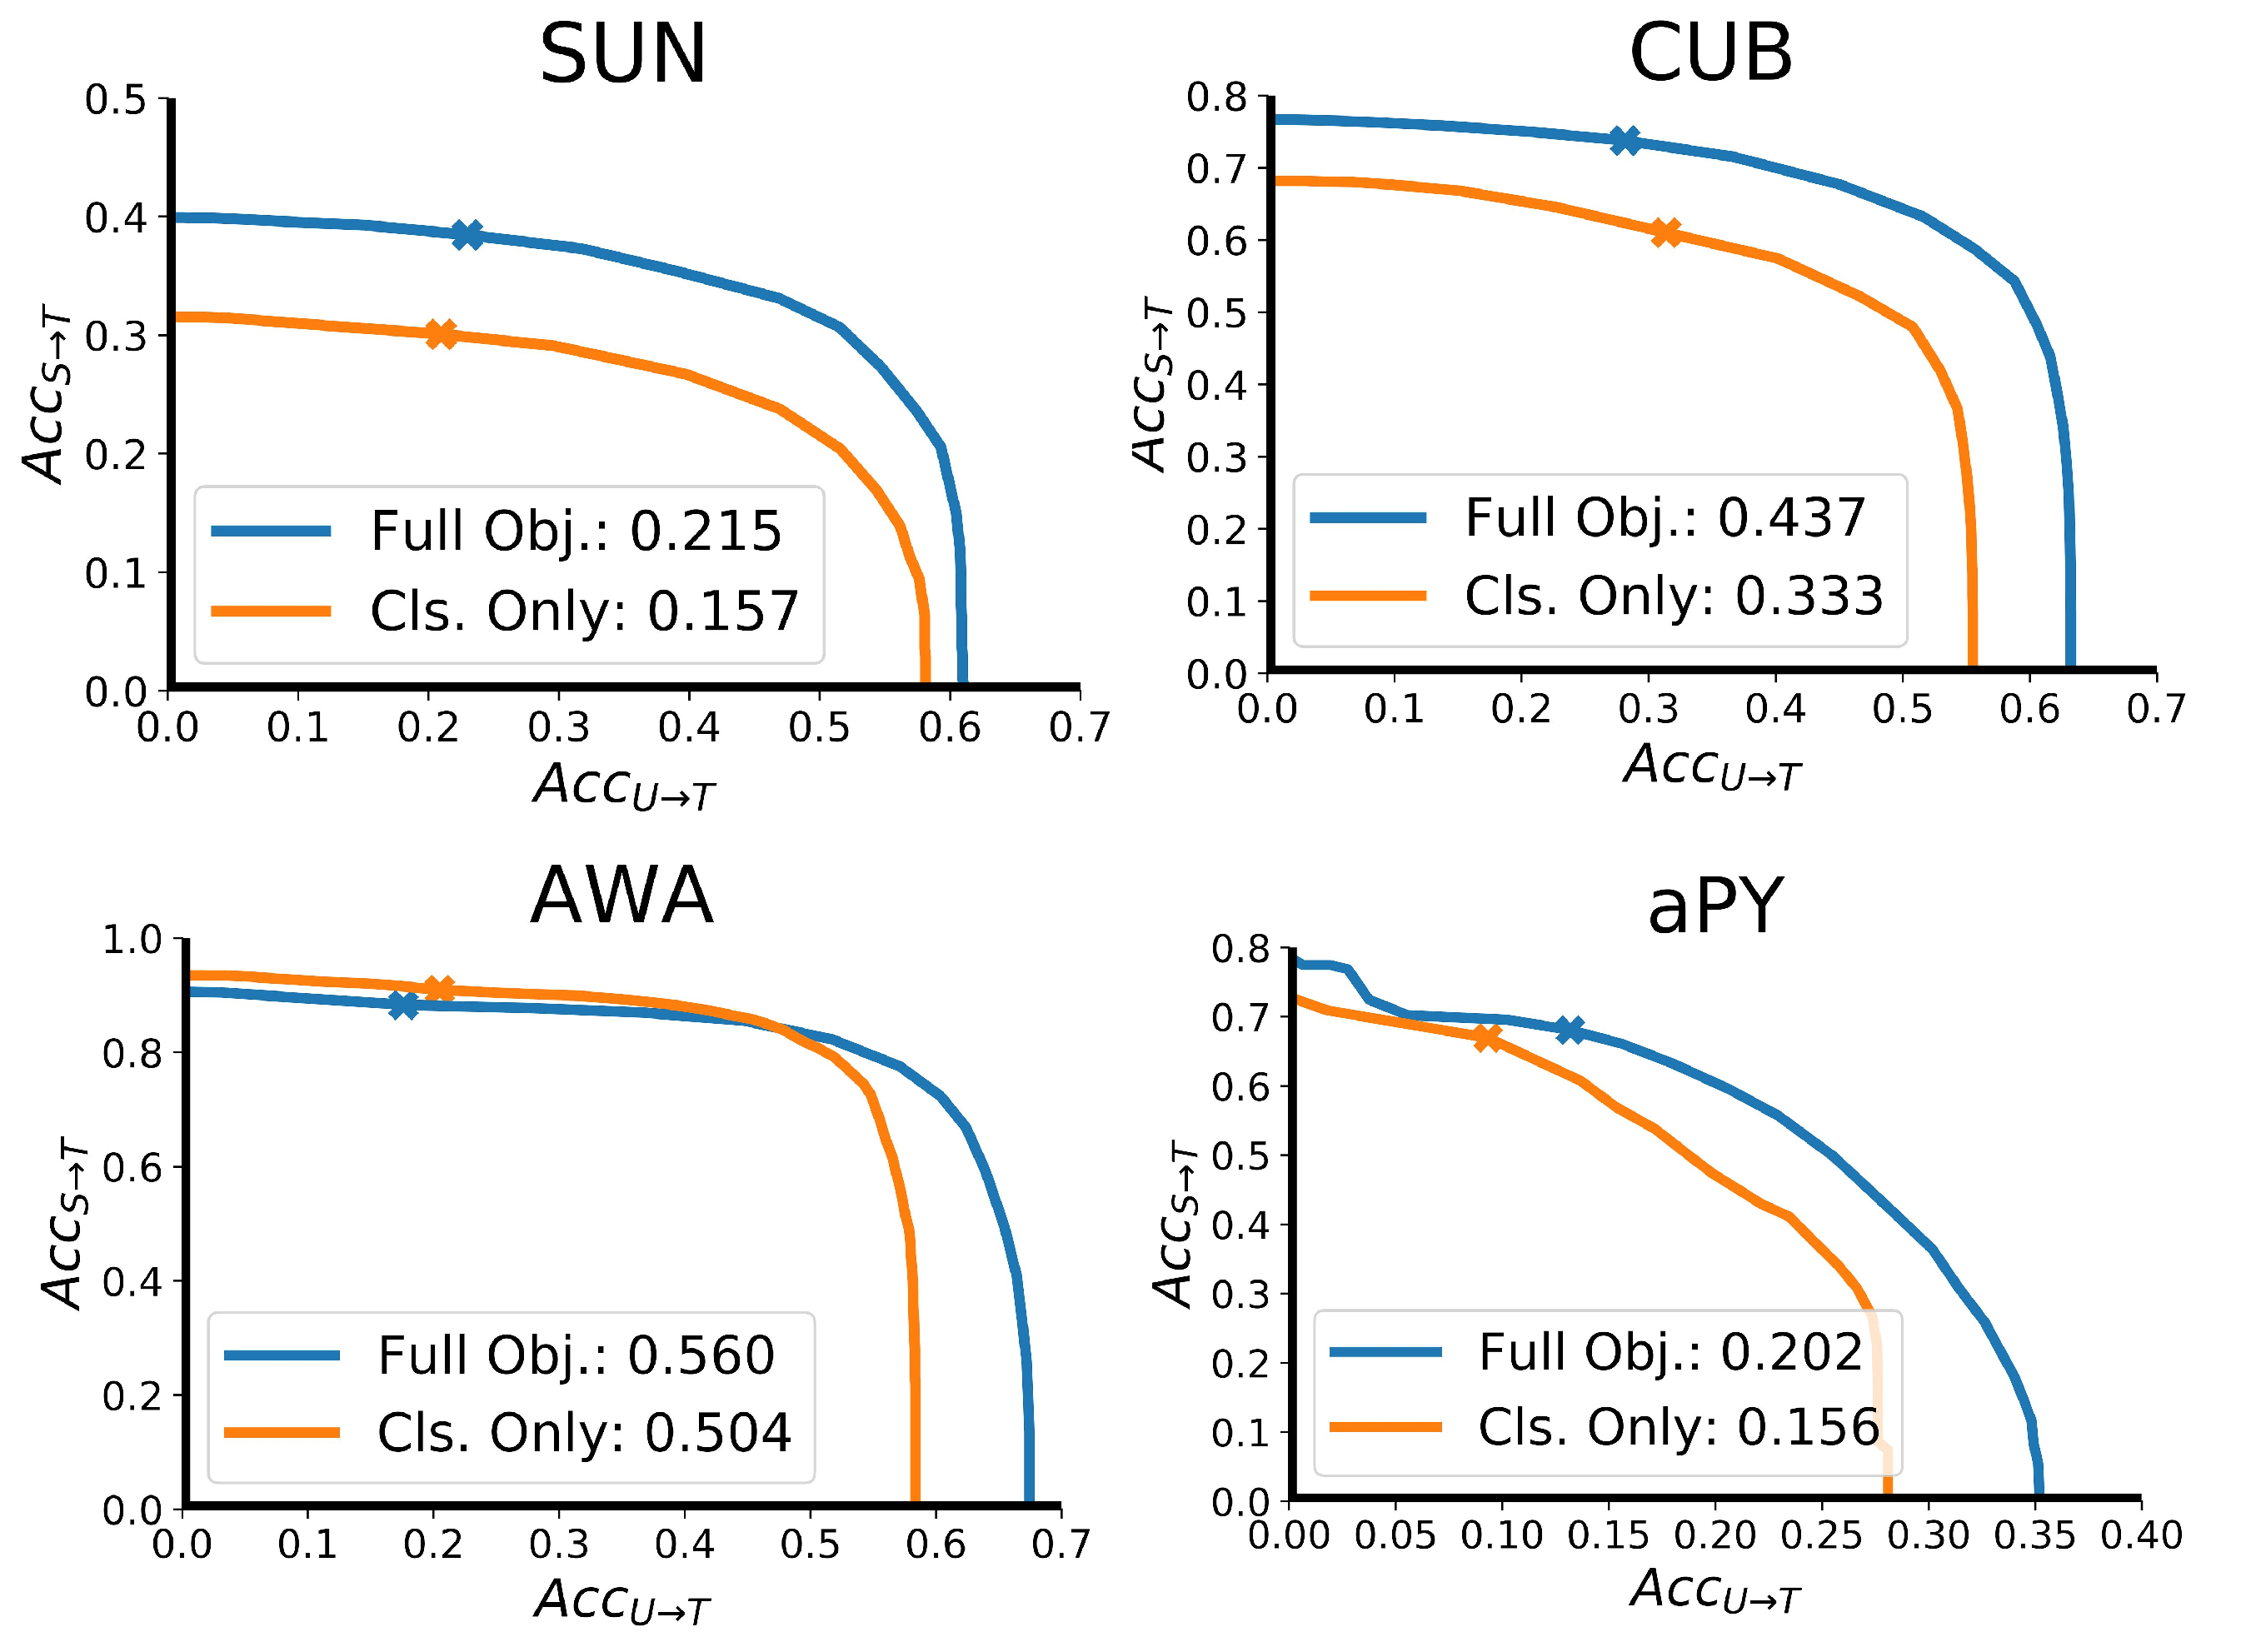
\includegraphics[width=0.7\linewidth]{chapter3/res/ausuc.pdf}
    \caption{在四个零样本分类数据集中的已见-未见准确率曲线下区域面积}
\label{ch3:fig:ausuc}
\end{figure}


\begin{table*}[htbp]
\centering
\scalebox{0.9}{
    \begin{tabular}{|l | c c c c|c c c c|}
    \hline
        Dataset & \multicolumn{4}{c}{\textbf{SUN}} & \multicolumn{4}{c|}{\textbf{CUB}} \\
    \hline
        Setting  & U$\to$U & U$\to$T & S$\to$T & H & U$\to$U & U$\to$T & S$\to$T & H \\ 
    \hline
        Cls. Only & 56.8 & 17.2 & 29.0 & 21.6 & 52.2  & 23.5 & 55.0 & 32.9 \\
        Full Obj. &\textbf{59.2} &  \textbf{24.9} & \textbf{38.6}& \textbf{30.3} & \textbf{55.4} & \textbf{34.7} & \textbf{70.6}  & \textbf{46.6} \\
    \hline
        Dataset & \multicolumn{4}{c}{\textbf{AWA}} & \multicolumn{4}{c|}{\textbf{aPY}} \\
    \hline
        Cls. Only & \textbf{60.2} &17.5 & 76.7& 28.5 & \textbf{35.8} & 5.5 & \textbf{72.9} & 10.2\\
        Full Obj. & 58.5 & \textbf{23.3} & \textbf{90.9} & \textbf{37.1} & 24.1 & \textbf{13.7} & 63.4 & \textbf{22.6} \\
    \hline
    \end{tabular}
}
\caption{SP-AEN在不同优化目标条件下的性能对比}
\label{ch3:tab:Full_Cls}
\end{table*}

如图~\ref{ch3:fig:ausuc}所示,蓝色曲线表示模型SP-AEN使用所有的优化目标(Full Obj.),而黄色曲线表示SP-AEN只使用分类任务优化目标(Cls. Only)。在所有的数据集中,SP-AEN(Full Obj.)相比于SP-AEN(Cls. Only)都可以显著提升模型性能。表~\ref{ch3:tab:Full_Cls}展示了两种模型的定量性能对比。从实验结果可以看出,当使用对抗学习优化目标和重建学习优化目标时,在所有的数据集中H值可以显著提升超过10\%。如图~\ref{ch3:fig:alpha_influence},当逐渐减少重建网络的权重$\alpha$(从左向右变化,红框为原始输入图像),图像重建的质量也逐渐降低。

\begin{figure}[ht]
    \centering
    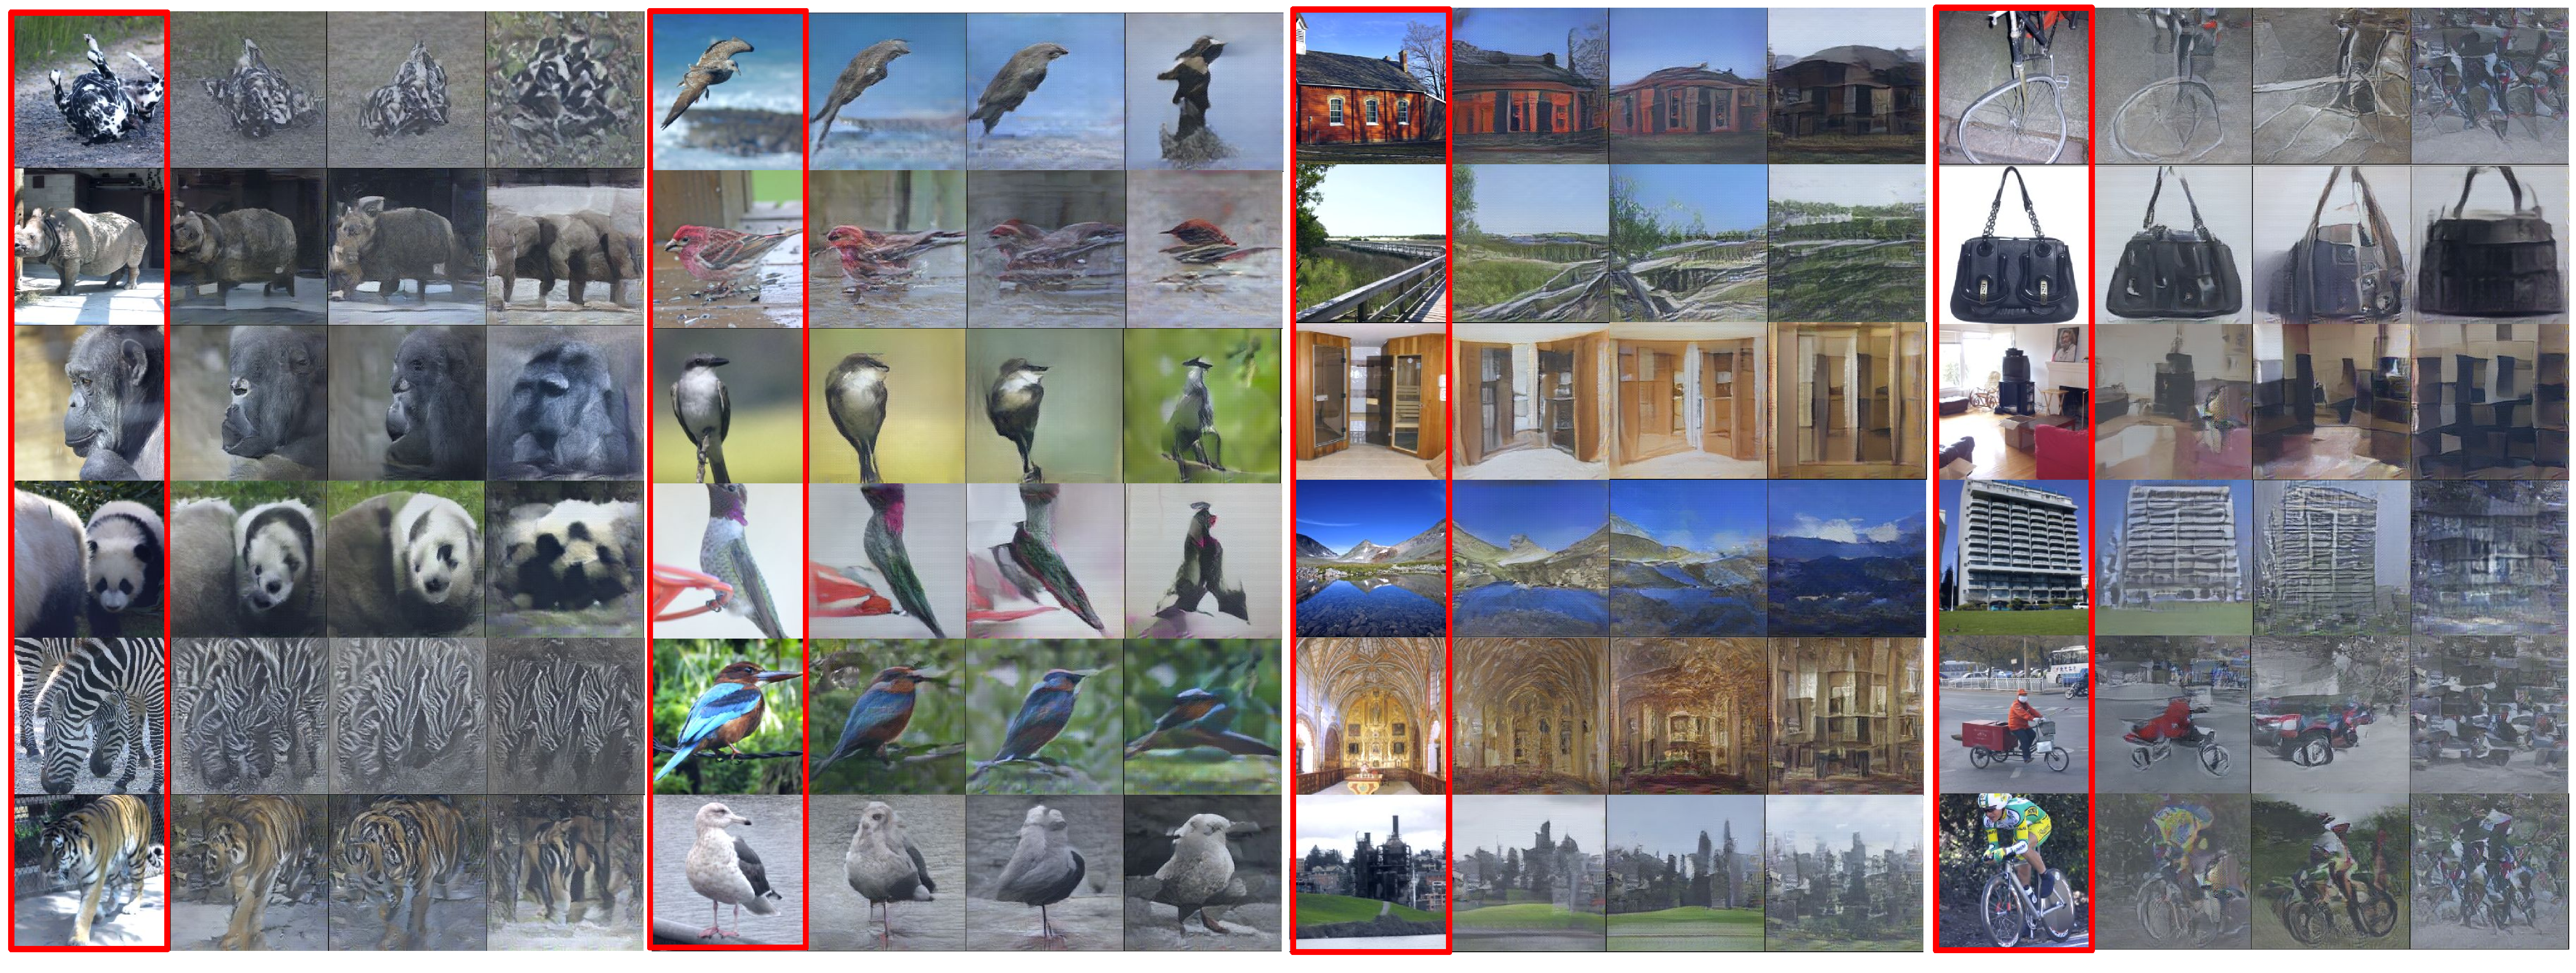
\includegraphics[width=0.99\linewidth]{chapter3/res/alpha_influence.pdf}
    \caption{图像重建结果随优化目标权重$\alpha$的影响}
\label{ch3:fig:alpha_influence}
\end{figure}


\section{本章小结}

本章我们提出了一个全新的零样本分类网络:属性保持对抗网络(SP-AEN),用于解决目前零样本分类方法中普遍存在的语义丢失的问题。SP-AEN主要通过两个设计来解决语义丢失:(1)引入一个独立的重建编码网络和重建解码网络,使得重建任务的优化目标不直接影响分类任务网络的优化。(2)通过引入对抗网络学习,实现重建网络编码向量和分类网络编码向量之间的知识迁移。在通用的四个标准零样本分类数据集中,我们通过大量的实验和可视化结果都证明了模型SP-AEN的有效性。


